
\documentclass[a4paper,12pt]{article}
\usepackage[utf8]{inputenc}
\usepackage[spanish,es-nodecimaldot]{babel}
\usepackage[T1]{fontenc}
\usepackage[intlimits]{amsmath}
\usepackage{graphicx}
\usepackage{a4wide}
\usepackage{float}
\usepackage[labelfont={bf},textfont={it}]{caption}
\usepackage{subcaption}


\usepackage{hyperref}
\hypersetup{ %
colorlinks=false  % false:boxedlinks ; true:coloredlinks
} %


\usepackage{tikz}
\usetikzlibrary{trees}
\usepackage{xcolor}

\graphicspath{{imagenes/}}

\title{\textsc{Modelo de Ising en 2D} \\ \vspace{2em} \Large{Introducción a la 
simulación computacional}}
\author{\small{ Pablo Bellino (pbellino@gmail.com)} \\
        \small{Luis María Pizarro (lpizarro@cnea.gov.ar)}}

\date{Octubre de 2015}


\begin{document}

%\inputencoding{latin1}

\maketitle

\begin{abstract}
Se implementó el algoritmo de Metrópolis para la simulación del modelo de Ising 
en 2D. Se calcularon las magnitudes del sistem (energía, magnetización, calor 
específico y suceptibilidad magnética) en función de la temperatura, donde se 
hizo manifiesto la $T_c$ donde se produce el cambio de fase. Se realizaron 
análisis cambiando el tamaño de la red para analizar los efectos de borde y 
finalmente se calcularon las funciones de auto-correlación temporal de la 
energía.
\end{abstract}


\section{Introducción}

El modelo de Ising fue formulado como una representación idealizada de un 
material ferromagnético. Se propone una red de spines con sus posiciones fijas, 
donde cada elemento podrá tomar sólo los valores $s_i=\pm1$. Se asume que la 
red es cuadrada y que la interacción ocurre solamente a primeros vecino. Bajo 
estas condiciones, se puede escribir el Hamiltoniano del sistema como:  

\begin{equation}{\label{eq:hamiltoniano}}
H = - J \sum_{\langle ij \rangle}^N s_is_j
\end{equation}

\noindent donde $\langle ij \rangle$ indica que la sumatoria se realiza con los 
sitios primeros vecinos, mientras que $J>0$ es la constante de acoplamiento de 
la interacción entre spines. Se omite el término de interacción con un cámpo 
magnético externo.

La magnetización del sistema para un dado estado se define como:

\begin{equation}
M = \mu \sum_{i=1}^N s_i
\end{equation}

\noindent donde $\mu$ es la permeabilidad magnética. Se dice que hay 
magnetización espontánea cuando $\langle M \rangle \neq 0 $ en ausencia de 
campo magnético externo. Para redes de dimensión $d \geq 2$ esto ocurre a 
temperaturas menores a cierta temperatura crítica $T_c$. Si $T>T_c$ el sistema 
será paramagnético con una magnetización media nula, mientras que para $T<T_c$ 
el sistema será ferromagnético y habrá magnetización esponánea. Este cambio de 
comportamiento del material es consecuencia de una transición de fase de 
segundo orden.

Se puede demostrar \cite{chand1987} que la temperatura crítica para una red 
cuadrada infinita, expresada en unidades adimensionales es:

\begin{equation}
\frac{k T_c }{J} = \frac{2}{ln(1+\sqrt{2})} \simeq 2.3
\end{equation}

Tanto el calor específico como la suceptibilidad magnética del sistema se 
definen en función de derivadas respecto de la temperatura. Derivada de la 
energía para el calor específico, y de la magnetización para la suceptibilidad. 
Sin embargo, en el trabajo se utilizará la relación de estas magnitudes con las 
fluctuaciones del sistema, ya que ello permite una mejor estimación de estas 
magnitudes. Entonces, el calor específico quedará definido como:

\begin{equation}\label{eq:cal_teo}
C  = \frac{1}{kT^2} \left(\langle E^2\rangle - \langle E \rangle^2\right)
\end{equation}

\noindent y la suceptibilidad magnética

\begin{equation}\label{eq:suce_teo}
\chi = \frac{1}{kT^2} \left(\langle M^2\rangle - \langle M \rangle^2\right)
\end{equation}

\noindent siendo $k$ la constante de Boltzman.

\subsection{Desarrollo de la simulación}

Se implementó el algoritmo de Metrópolis para obtener una colección 
representativa de distintos estados del sistema del ensamble canónico. Se 
utilizaron condiciones periódicas de contorno con el fin de suprimir los 
efectos de borde del sistema. De esta manera se pretende simular el seno del 
material en un sistema infinito.

Se escribió el programa \texttt{ising} de acuerdo al siguiente algoritmo:

\renewcommand{\theenumi}{\roman{enumi}}
\begin{enumerate}
	\item Se elije un estado inicial del sistema. Esto puede realizarse al 
	azar, haciendo que cada spin tome valores $s_i=\pm1$. También se permitió 
	que el estado inicial fuera leido de un archivo.
	\item Se elije aleatoriamente un spin de la red.
	\item Se calcula la energía que tendría el nuevo estado si se invirtiera el 
	spin seleccionado. Se calcula la diferencia de energía respecto al estado 
	previo.
	\item Si la diferencia de energía es negativa, se acepta el estado. 
	\item Si la deferencia de energía es positiva se acepta el nuevo estado 
	propuesto con probabilidad $exp(-\Delta E/kT)$. Para ello se muestrea un 
	número $r$ al azar con distribución uniforme $\mathcal{U}(0,1)$. Si $r< 
	exp(-\Delta E/kT)$ se acepta el estado, de lo contrario es rechazado.
    \item En caso de haber sido aceptado se invierte el spin y se 
    calcula la magnetización. Se guardan los datos de $E$y $M$.
    \item Se vuelve al punto (\textrm{II}) hasta haber completado $K$ ciclos 
    del 
    algoritmo.
\end{enumerate}

\section{Medición de observables}

En esta sección se describirá la metodología utilizada para la estimación de 
los observables una vez termalizado el sistema a la temperatura de trabajo.

Para una determinada corrida $r$ del programa \texttt{ising}, se obtiene la 
energía y la magnetización realizando un promedio sobre todos los valores 
obtenidos en cada paso del algoritmo de Metrópolis:

\begin{subequations}
   \begin{align}
  E^r \equiv &\frac{1}{K}\sum_{i=1}^K E^r_i 
  \label{eq:E_prom}\\
  M^r \equiv & \frac{1}{K}\sum_{i=1}^K M^r_i 
  \label{eq:M_prom}
   \end{align}
\end{subequations}

\noindent donde $K$ son la cantidad total de pasos realizados.

Las estimaciones del calor específico y de la suceptibilidad magnética para una 
corrida $r$ se realizaron de manera similar, teniendo en cuenta las expresiones 
teóricas dadas de las ecuaciones \eqref{eq:cal_teo} y \eqref{eq:suce_teo} 
respectivamente:

\begin{equation}
 C^r \equiv  \frac{1}{kT^2} \frac{1}{\sqrt{K-1}} \sum_{i=1}^K \left(
 E_i^r - E^r \right)^2
\end{equation}

\begin{equation}
 \chi^r \equiv  \frac{1}{kT} \frac{1}{\sqrt{K-1}} \sum_{i=1}^K \left(
 M_i^r -  M^r \right)^2
\end{equation}

Para tener un resultado estadísticamente relevante, se efectuaron varias 
corridas con los mismos parámetros. Esto permitió obtener el resultado final de 
las magnitudes con su respectivo error. Llamando $N_r$ a la cantidad de 
repeticiones realizadas a una dada temperatura los valores medios y 
desviaciones estándar se definieron como:

\begin{subequations}
\begin{align}
X & \equiv \langle X^r \rangle = \frac{1}{N_r} 
\sum_{r=1}^{N_r} X^r \\
\sigma(X) & \equiv \frac{\sigma(X^r)}{\sqrt{N_r}} =  \sqrt{\frac{1}{N_r(N_r-1)} 
\sum_{i=1}^{N_r} \left( 
 X^r -  X \right)^2}
\end{align}
\end{subequations}

\noindent donde $X^r$ puede ser cualquiera de los cuatro observables estimados 
en cada corrida: $E^r$, $M^r$, $C^r$ ó $\chi^r$. En esta última expresión, se 
utiliza el hecho de que la distribución del valor medio de $Xr$ tiende a una 
Gaussiana debido al Teoréma Central del Límite.



\section{Descripci\'on del sistema de c\'alculo}


Se desarrollo un c\'odigo de c\'alculo en Fortran y dos c\'odigos
en python uno  de pre y el otro de postprocesamiento. Tanto el código de 
preprocesamiento, 
como el código de postprocesamiento, comprenden varios módulos responsables de distintas
tareas.

El proyecto se encuentra bajo control de versión en un repositorio \textbf{git} de CNEA
y se obtiene con los permisos adecuados haciendo:

\begin{verbatim}
> git clone https://lpizarro@scmmanager.dcap.cnea.gov.ar/scm/git/SimRui
\end{verbatim}

Una vez cloneado el repositorio, para acceder al código, hacer:

\begin{verbatim}
  > cd FORTRAN/dinmod
\end{verbatim}

El c\'odigo fuente del programa \textbf{\textit{dinmod.f90}}, se encuentra en la carpeta
\textbf{src/}, su compilación se hace con el sistema \textbf{cmake} y depende
de un conjunto de módulos que se encuentra en la carpeta \textbf{libs}.

Para compilarlo hay que corre el script \textbf{\textit{instalar.sh}}:

\begin{verbatim}
  > ./instalar.sh 
\end{verbatim}

esa operación crea un directorio  \textbf{build/bin/} donde se encuentran todos
los elementos necesarios para hacer las corridas del programa.

\subsection{Código FORTRAN}

\subsubsection{Módulos  utilizados}

La carpeta \textbf{libs/} contiene los módulos utilizados por el sistema, ellos son:

\paragraph{\underline{\textit{inic\_fin.f90}}}:

Un conjunto de subrutinas para inicializar y finalizar el sistema de cálculo:

\begin{itemize}
  \item  Inicializa parametros para la g(r)
  \item  Calcula el radio de corte y el desplazamiento de potencial

  \item Inicializa las velocidades

  \item Inicializa posición aleatoria dentro de la caja

  \item Integración de las ecuaciones de movimiento - minimización energía

  \item Subrutina de finalización  del cálculo
\end{itemize}

\paragraph{\underline{\textit{procesamiento.f90}}}:

 Se hace estadistica sobre vectores y se escriben  resultados, se calculan 
 valores medios y desviacions estándares
 luego  se escriben los resultados al archivo \textbf{\textit{val\_medios.dat}}

\paragraph{\underline{\textit{types.f90}}}:

En este módulo se encuentran las definiciones de tipos fundamentales que se usan 
en todo el sistema.

\paragraph{\underline{\textit{integra.f90}}}:

 En este módulo se tiene la rutina que  integra las ecuaciones dinámicas 
 con el algoritmo de velocity-verlet y otra que aplica las condiciones períodicas 
 de contorno en forma vectorial.

\paragraph{\underline{\textit{constants.f90}}}:

 En este módulo se definen constantes que se utilizan en otros módulos. 

\paragraph{\underline{\textit{estadistica.f90}}}:

Un conjunto de subrutinas para análisis estad\'istico para:
\begin{itemize}
	\item{Calcular los datos para graficar un histograma - de forma vectorial},  
	\item{calcular los datos para graficar un histograma - punto por punto}.

	\item{Promedio y desviacion estandar de forma iterativa.}

 Se evita cargar en memoria todos los datos a la vez. Se leen de a uno y se 
 calculan el promedio y la varianza normalizada con \textit{sqrt(1-N)} recursivamente. 

 ADVERTENCIA: El método usado tiene problemas de redondeo para N muy grande.
 Se tendria que modificar el algoritmo pararealizar el promedio (i.e de a pares)
 Sin embargo, trabajando con doble precision se mejora bastante sin hacer nada.

 \item{Promedio y desviacion estandar vectorizado.}

 La desventaja es que debe cargar al archivo completo en memoria. La ventaja es
 que tiene menos errores de redondeo.

 \item{Promedio y desviacion estandar vectorizado directo.}

 La desventaja es que debe cargar al archivo completo en memoria. La ventaja es
 que tiene menos errores de redondeo.
 Es igual a \textit{vector\_mean\_var()} solo que opera sobre el vector de entrada
 y no sobre el archivo con los datos

\end{itemize}

\paragraph{\underline{\textit{globales.f90}}}:

En este  m\'odulo se encuentran  todas las variables globales del programa.
	
\paragraph{\underline{\textit{io\_parametros.f90}}}:

Un m\'odulo para el manejo de la entrada y las salidas de los datos del programa.

Se encuentran  subrutinas para:
\begin{itemize}
 \item Leer los datos de entrada del problema.

 \item Esbribir posiciones para visualizar trayectorias.

 \item Esbribir un vector 1D a un archivo en columnas.

 \item Esbribir un vector 2D a un archivo en columnas.

 \item Esbribir estados de posicion y velocidad.

 \item Leer estados de posicion y velocidad.

\end{itemize}

\paragraph{\underline{\textit{usozig.f90}}}: 

En este m\'odulo se ecuentran las subrutinas que usan ziggurat y que
son usadas en el programa principal, \textbf{\textit{dinmod}}.
					
\paragraph{\underline{\textit{ziggurat.f90}}}:

Módulo para la generaci\'on de n\'umeros aleatorios. 

\paragraph{\underline{\textit{mediciones.f90}}}:

En este m\'odulo  se encuentran rutinas de c\'alculo del
sistema.

\begin{itemize}
	\item Calcula la fuerza y la energía potencial del potencial de L-J

	\item Termostato de Langevin. Agrega la parte estocástica a la fuerza de cada partícula

	\item Calcula la presion en base al teorema del virial 

	\item Calcula la anergia cinetica total del sistema

	\item Calcula temperatura instantanea de las partículas dentro de la caja 
\end{itemize}

\paragraph{\underline{\textit{utils.f90}}}:

\begin{itemize}
   \item Función para medir el wall-time

 \item   Subrutina para inicializar parametros en el caso de haber compilado con OpenMP

 \item   Subrutina para imprimir con formato por pantalla un array 3D en lineal 

\end{itemize}


\subsection{Código Python}

El control de las corridas del código en FORTRAN se hace desde scripts en el lenguaje
de alto nivel  \href{http://www.python.org/}{phyton}. 

Para eso hay que parametrizar adecuadamente el sistema en \textbf{\textit{parametros\_t.py}}
\textbf{\textit{parametros\_rho.py}}, en un caso se parametriza la dependecia en temperaturas
de las corridas y en el otro la dependencia en la densidad.
 
Los comentarios del módulo explican el fin de cada una de las variables globales python.

\begin{verbatim}

###############################################################################       
#   PARAMETROS DE ENTRADA PARA CORRER A DISTINTAS TEMPERATURAS
###############################################################################
# Número de partículas
N_part = 200
# Densidad de partículas
Rho = 0.3
#------ Barrido de temperaturas
# Temperatura mínima
Temp_min = 0.7
# Temperatura máxima
Temp_max = 1.4
# Paso de temperatura
dTemp = 0.25
# Agrego el detalle cerca de la temperatura crítica
#T_detail_min = 2.10
#T_detail_max = 2.50
#dT_detail = 0.02
# abs(K_grab) Cada cuántos puntos se quiere grabar el archivo temporal
# K_grab < 0 especifica que no se grabe ningún archivo temporal
N_grab = 10
# Paso temporal de integración
dt = 0.001
# Número de pasos para la primer corrida (termalización)
N_term = 1000
# Número de pasos para la segunda corrida (medición)
N_medi = 2000
# Número de corridas para cada temperatura
Nrun = 8
#
# FIN PARAMETROS DE ENTRADA
###############################################################################

\end{verbatim}

\subsection{Corridas del programa}

El programa se puede correr en serie, o en paralelo usando  \href{http://openmp.org/}{openMP} 
(paralelización multi-core en memoria compartida)o  \href{http://www.open-mpi.org/}{MPI} (Message Passing Interface).

\subsubsection{Corridas en serie}
Para correr en serie se debe poner en el script \textbf{\textit{instalar.sh}}
el parámetro -\textbf{\textit{Dopenmp=OFF}} del comando cmake.

\subsubsection{Corridas con openMP}
Para correr en serie se debe poner en el script \textbf{\textit{instalar.sh}}
el parámetro -\textbf{\textit{Dopenmp=ON}} del comando cmake.

\subsubsection{Corridas con MPI}

Para correr con MPI se usa 
el paquete \href{http://mpi4py.scipy.org/} {\textbf{mpi4py}} ,  desarrollado.
Un script en python distribuye el trabajo entre varios nodos  

y luego hacer, para correr la versión serie:

\begin{verbatim}
  > cd bin/
  > python corridas.py
\end{verbatim}

o si se quiere correr la versión paralelo:

\begin{verbatim}
  > cd bin/
  > mpirun.mpich -n 8 python corridas_paralelos.py
\end{verbatim}

Luego de una corrida en una serie de temperaturas, queda una estructura de directorios
como la que se muestra en \eqref{fig:arboldir}, con la información necesaria 
para postprocesar
los resultados y obtener los valores de las mediciones en función de la temperatura.

\tikzstyle{every node}=[thick,anchor=west, 
font={\scriptsize\ttfamily}, inner sep=2.5pt]
\tikzstyle{selected}=[draw=blue,fill=blue!10]
\tikzstyle{root}=[draw=blue, fill=blue!30]

\begin{figure}[H]
\begin{center}
\begin{tikzpicture}[%
    scale=.7,
    grow via three points={one child at (0.5,-0.65) and
    two children at (0.5,-0.65) and (0.5,-1.2)},
    edge from parent path={(\tikzparentnode.south) |- (\tikzchildnode.west)}]
  	\node [root] {bin}
  	child { node [red] {dinmod}}
  	child { node [red] {corridas\_paralelo\_t.py}}
  	child { node [red] {corridas\_paralelo\_rho.py}}
  	child { node {tablas\_temperatura.dat}}
	child { node {energia\_pot\_min.dat }}
	child { node {energias.dat }}
	child { node {estados.dat}}
	child { node {parametros.dat}}
	child { node {presion.dat}}
	child { node {seed.dat}}
	child { node {temperatura.dat}}
  	child { node {val\_medios.dat}}
    child { node [selected] {temperatura\_0.7}
      child { node {parametros.dat}}
      child { node {estados.dat}}
      child { node {runs\_estadistica.dat}}
      child { node [selected] {RUN00}
	     child { node {val\_medios.dat}}
	     child { node {estado.dat}}
	     child { node {ultimo\_estado.dat}}
      }
      child { node at(0,-1.8) [selected] {RUN01}}
      child { node at(0,-1.9) [selected] {RUN02}}
      child { node at (0,-2.0) {\dots}}
    }       
    child { node at (0,-5.5) [selected]{temperatura\_0.75}}
    child { node at (0,-5.8)[selected] {temperatura\_0.8}}
    child { node at (0,-6.1) {\dots}};
\end{tikzpicture}
\end{center}

\caption{Esquema de carpetas y archivos que se obtienen al realizar una corrida 
completa haciendo estadísticas en cada temperatura.}
\label{fig:arboldir}
\end{figure}

Una vez que se terminan los cálculos para todas las temperaturas,  en 
la carpeta \textbf{bin/}, se corre:

\begin{verbatim}
  > python grafico_tablas.py 
\end{verbatim}

para obtener los gráficos de las medidas fundamentales del sistema.

Si se quieren obtener los gráficos de las correlaciones a distintas temperaturas, 
se debe correr:

\begin{verbatim}
  > python correlaciones.py 
\end{verbatim}

\subsection{C\'odigo dinmod}

\subsubsection{Par\'ametros de entrada}

El programa \textbf{\textbf{dinmod}} lee la configuraci\'on de una corrida del 
archivo \texttt{parametros.dat} que tiene que estar en la carpeta donde se
corre \textbf{\textbf{dinmod}}.

El archivo \texttt{parametros.dat} tiene la forma: 

\begin{verbatim}
     T  Npart  L dt Ntime  sigma epsilon masa Nmed
     gamma
\end{verbatim}

Donde Npart
Es el número de partículas del sistema, \textit{T} la temperatura de la corrida,
\textit{L} una de las dimensiones de la caja, \textit{dt} el paso de tiempo de integración,
\textit{Ntime} la cantidad de pasos de integración,
\textit{sigma} el parámetro $\sigma$ del potencial de Lennard-Jones,
\textit{epsilon} el parámetro $\epsilon$ del potencial de Lennard-Jones,
\textit{masa} la masa de la partícula,
\textit{Nmed} cada cuentas mediciones se graban datos,
\textit{gamma} el parámetro $\gamma$ del termostáto de Langevin,

Un ejemplo de ese archivo es:

\begin{verbatim}
   6.0 200 5.5032 0.001 20000 1.0 1.0 1.0 1
   0.5
\end{verbatim}

\paragraph{Preprocesamiento en python}

En la carpeta \textbf{src/} el archivo \texttt{parametros.py} contiene la 
parametrizaci\'on de los scripts en python que permiten correr el sistema en 
serie (ver \eqref{serie}), 
o en paralelo (ver \eqref{paralelo}).
El preprocesamiento en python, permite definir una zona de c\'alculo de paso
de temperatura fino. Es decir se puede parametrizar un paso de temperatura de
$0.1$ para todo el rango de temperatura y dentro de ese rango definir una zona
donde el paso de temperatura puede ser menor, ej. $\Delta T = 0.02$. Para 
lograr una mejor resoluci\'on
en esa zona.

En particular en este c\'alculo se uso para explorar con m\'as detalle la zona
cr\'itica.

El preprocesamiento en python, crea el archivo \texttt{parametros.dat}, 
 corre el programa de ising a distintas temperaturas y crea una carpeta para 
 cada temperatura. En cada una de esas carpetas, a su vez, crea Nruns carpetas 
 para hacer estadística y obtener los valores con sus respectivos errores.
 
  En cada temperatura, se utiliza el valor final de la temperatura anterior.
  Arbitrariamente, se toma el valor final de RUN00 como el valor inicial de
  todas las corridas a la siguiente temperatura (menor).
 

\subsubsection{Salida del programa}

Los resultados los guarda en el archivo \texttt{tablas\_temperatura.dat}.

Cada fila de \texttt{tablas\_temperatura.dat} representa los resultados a una 
dada temperatura con sus respectivos errores. Las columnas son:

\begin{verbatim}
  T <E> std(E) <M> std(M) <c> std(c) <suc> std(suc) <acept> std(acept)
\end{verbatim}

Donde:

\begin{itemize}
  \item $T$: temperatura de la corrida 
    \item $<E>$: Energ\'ia media calculada
    \item  $std(E)$: desviaci\'on standard de la energ\'ia calculada

    \item $<M>$: Magnetizaci\'on media calculada
    \item  $std(M)$: desviaci\'on standard de la Magnetizaci\'on calculada


    \item $<c>$: Capacidad calor\'ifica media calculada
    \item  $std(c)$: desviaci\'on standard de la Capacidad calor\'ifica calculada

    \item $<suc>$: Susceptibilidad magn\'etica media calculada
    \item  $std(suc)$: desviaci\'on standard de la Susceptibilidad magn\'etica calculada


    \item $<acept>$: Aceptaci\'on media calculada
    \item  $std(acept)$: desviaci\'on standard de la Aceptaci\'on calculada
\end{itemize}


\subsection{Corridas en serie}\label{serie}
El módulo python \texttt{corridas.py}, es el que tiene la capacidad de correr
el código de cálculo en una máquina con un único núcleo. Parametrizando 
adecuadamente \texttt{parametros.py} se logran tiempos de corrida razonables en 
una máquina con un único procesador. El parámetro que permite acelerar la 
velocidad de procesamiento, es el que indica cada cuantos pasos Monte Carlo se 
quieren grabar las energías.

\subsection{Corridas en paralelo}\label{paralelo}

El módulo python \texttt{corridas\_paralelos.py}, es el que tiene la capacidad 
de correr en una máquina con varios núcleos.

El código se paraleliza usando el paquete \href{http://mpi4py.scipy.org/} {\textbf{mpi4py}} ,  desarrollado por Lisandro Dalcin.
De esa manera lo que se hizo, es paralelizar desde python y no desde Fortran.

El criterio utilizado para paralelizar es hacer en simultaneo  las corridas a 
una dada temperatura. 
Una vez que terminan los cálculos a una dada temperatura, se hacen los cálculos 
en la próxima temperatura con el estado final de la temperatura anterior.

Este diseño permitió hacer cálculos en sistemas de mayor tamaño, lograndose llegar a dimensiones
de 100x100. De esa manera se obtuvieron las curvas que muestran el comportamiento del sistema en
tamaños mayores a 20x20.


\section{Resultados}

\subsection{Termalización del sistema}

Para obtener resultados a una dada temperatura, se realizaron, en verdad dos 
corridas. La primera de ellas consistió en llevar al sistema, desde su estado 
inicial, hasta el estado de equilibrio. A ete proceso se lo denomina 
termalización. Luego, la segunda corrida comienza con el último estado obtenido 
obtenido aquí para la parte de mediciones. En la Figura \ref{fig:terma_01} se 
muestran algunos ejemplos de cómo es el proceso de termalización a distintas 
condiciones.

\begin{figure}\label{fig:terma_01}
	\begin{center}
	\begin{subfigure}{.49\textwidth}
		\centering
      	\includegraphics[scale=0.4]{{terma_t0.5_ei_rand}.pdf} \\
     	 \caption{$T=0.5$ Estado inicial aleatorio}\label{fig:terma.t05_rand}
	\end{subfigure}
	\begin{subfigure}{.49\textwidth}
		\centering
     	 \includegraphics[scale=0.4]{{terma_t5.0_ei_up}.pdf} \\
      	\caption{$T=5.0$ Estado inicial con $s_i=1$}\label{fig:terma.t50_up}
	\end{subfigure}
	\end{center}
	\caption{Proceso de termalización con distintas temperaturas y estados 
	iniciales}
\end{figure}

El criterio para saber cuándo se llegó al estado de equilibrio es fácil de 
obtener visalmente viendo la evolución de la energía y la magnetización en cada 
paso el algoritmo. Sin embargo, al querer automatizar el proceso de ejecución 
del programa, se debe fijar un criterio tamibén automático para deteminar el 
punto de termalización.

En este trabajo el criterio utilizado, fue realizar varias corridas a 
distintas temperaturas y distintas configuraciones iniciales, y registrar 
manualmente el número de pasos necesarios para llegar al equilibrio. Luego, 
entre todos los valors obtenidos se definió que la cantidad de pasos para la 
termalización $K_{term}$ sea diez veces el máximo valor obtenido. En la 
práctica, para una red de 20x20, se tomaron $K_{term}=50000$. En las Figuras 
\eqref{fig:terma_01} y \eqref{fig:terma_02} se muestran cuatro situaciones 
cambiando la temperatura de trabajo y el estado inicial de dónde se parte.

\begin{figure}\label{fig:terma_02}
	\begin{center}
	\begin{subfigure}{.49\textwidth}
		\centering
      	\includegraphics[scale=0.4]{{terma_t3.0_ei_rand}.pdf} \\
     	 \caption{$T=3.0$ Estado inicial aleatorio}\label{fig:terma.t3_rand}
	\end{subfigure}
	\begin{subfigure}{.49\textwidth}
		\centering
     	 \includegraphics[scale=0.4]{{terma_t3.0_ei_up}.pdf} \\
      	\caption{$T=3.0$ Estado inicial con $s_i=1$}\label{fig:terma.t3_up}
	\end{subfigure}
	\end{center}
	\caption{Termalización a la temperatura $T=3.0$ partiendo de dos 
	configuraciones de spines distintas}
\end{figure}

Esta forma de obtener los pasos de termalización resulta mucho mayor que el 
necesario, ya que en las corridas efectuadas siempre se tomó el estado final de 
la corrida efectuada a una temperatura anterior (salvo la primer corrida, a 
temperaturas altas, que se tomó un estado inicial arbitrario).

\newpage

\subsection{Dependencia con la temperatura del sistema}

En esta parte se describen los resultados obtenidos al repetir las simulaciones 
con distintas temperaturas de trabajo. El barrido de temperaturas se realizó de 
forma automática con un $\Delta T = 0.1$ (en unidades adimensionales) y se 
redujo a $\Delta T = 0.02$ en la zona cercana a la temperatura crítica, para 
obtener mayor detalle. En todos los casos cada corrida fue de $K=1e7$ puntos y 
se realizaon $N_r=40$ corridas por cada temperatura.

En la Figura \eqref{fig:val_medios} se muestran los resultados de la energía y 
la magnetización con sus respectivos errores para una red de spines de 20x20. 
Especialmente en el gráfico de la magnetización, se hace evidente el cambio de 
fase cercano a la temperatura crítica donde para valores menores, aparece 
magnetización espontánea.

\begin{figure}[H]
    \begin{center}
      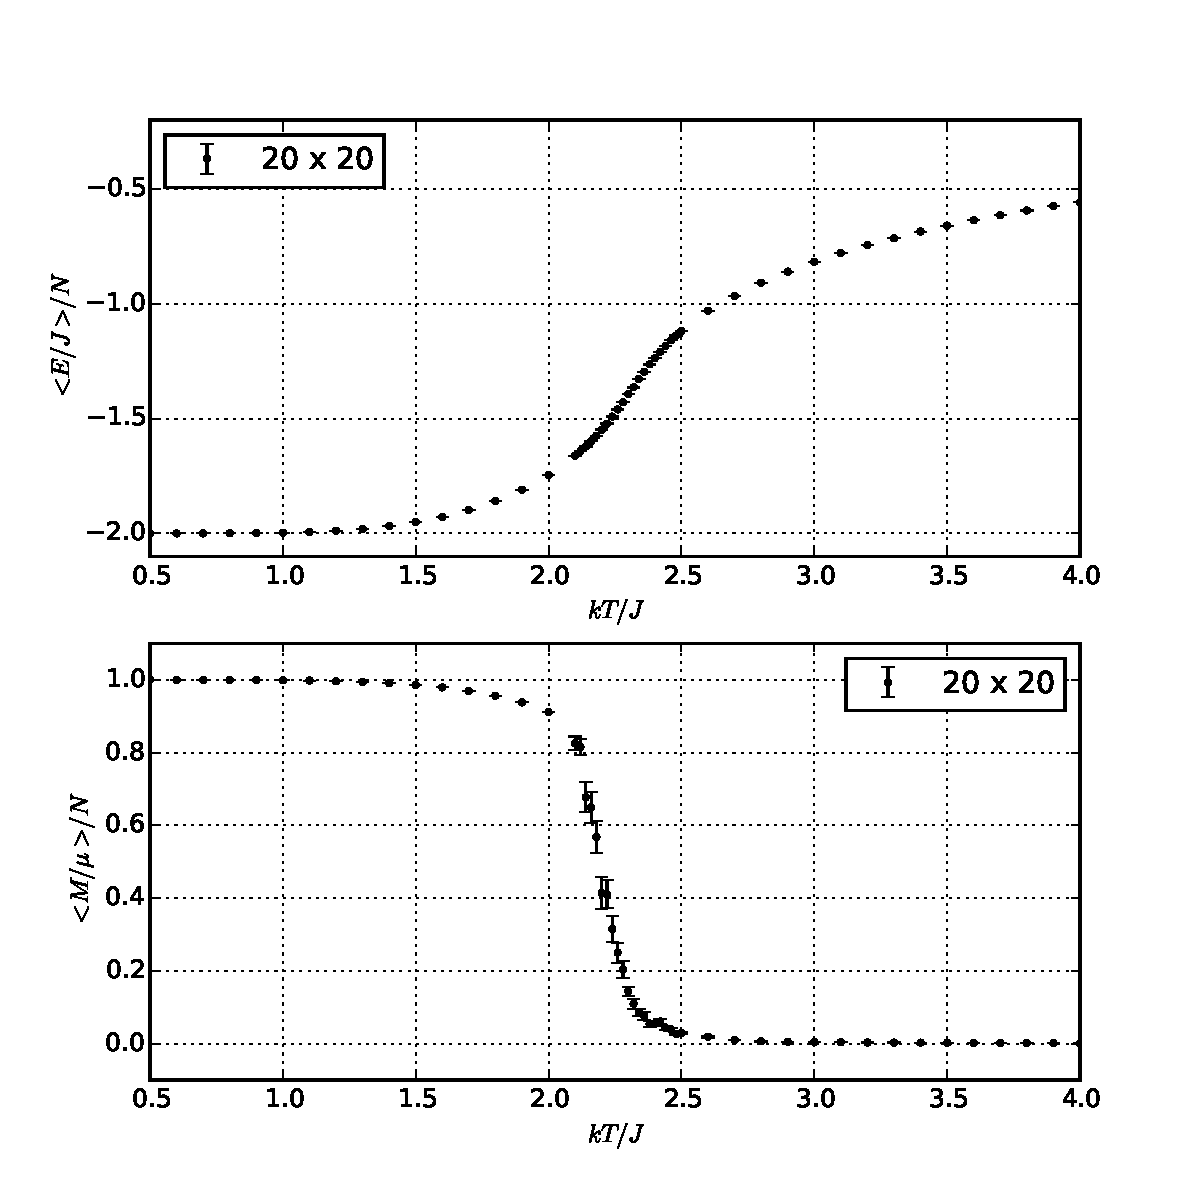
\includegraphics[scale=0.7]{val_medios.pdf} \\
      \caption{Valores de energía y magnetizació por spin, para 
      las distintas temperaturas simuladas}\label{fig:val_medios}
    \end{center}
\end{figure}

En la figura \eqref{fig:fluctuaciones} se muestran los gráficos 
correspondientes al calor específico y a la suceptibilidad magnética. Cerca de 
la temperatura crítica se observan un aumento de ambas magnitudes 
(teóricamentep ara un sistema infinito hay una divergencia). En esa misma zona, 
se observó también un aumento del error en los estimadores, producto de las 
grandes fluctuaciones con que evolucionaba el sistema. A partir de estos 
gráficos puede determinarse la temperatura crítica del sistema como el máximo 
de ambas curvas.

\begin{figure}[H]
    \begin{center}
      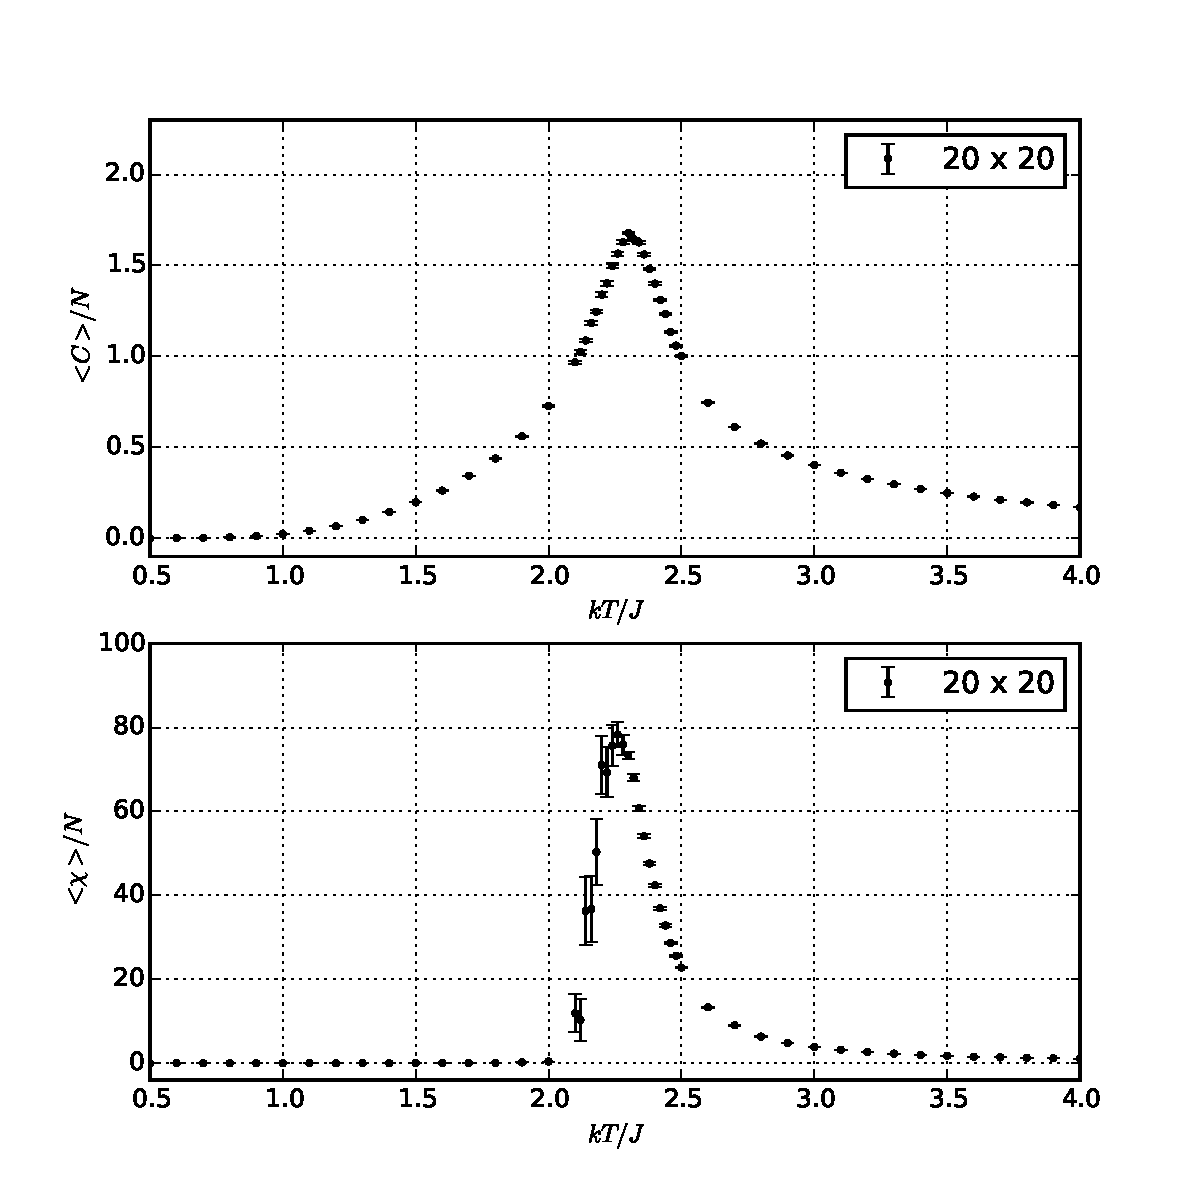
\includegraphics[scale=0.7]{fluctuaciones.pdf} \\
      \caption{Valores de calor específico y suceptibilidad magnética por spin 
      en función de la temperatura} \label{fig:fluctuaciones}
    \end{center}
\end{figure}

Finalmente, se muestra en la Figura \eqref{fig:aceptaciones} el porcentaje de 
aceptaciones a lo largo de todos los pasos del algoritmo de metrópolis, en 
función de la temperatura de trabajo. Esta curva, como es de esperar, sigue un 
comportamiento similar a la curva de energía (depende intrínsecamente de ella). 
Se observa que a bajas temperaturas, la mayoría de los estados propuestos son 
rechazados, ya que el sistema prefiere tener todos sus spines en la misma 
direccion. Aumentando la temperatura, el porcentaje de aceptaciones comienza a 
incrementarse haciendo que el sistema pueda recorrer mayor cantidad de estados.

\begin{figure}[H]
    \begin{center}
      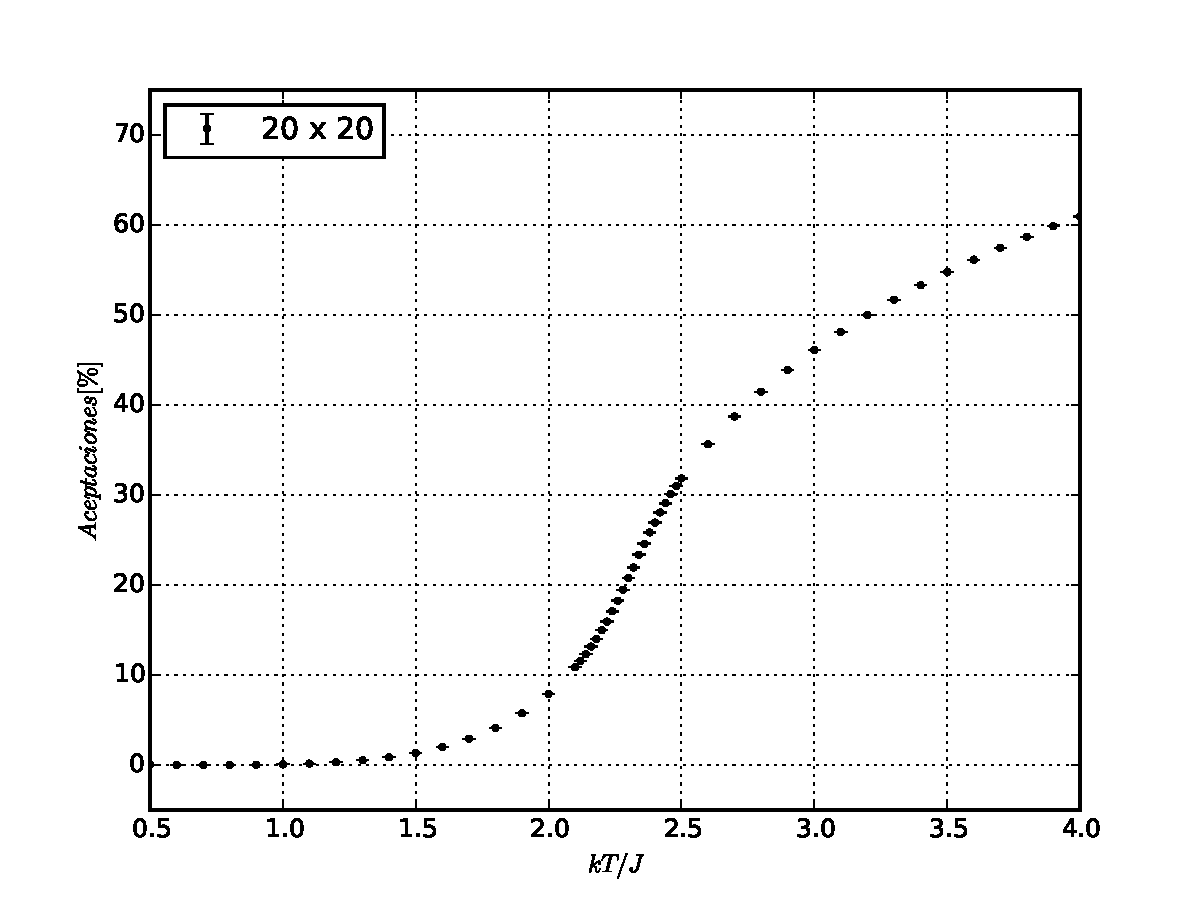
\includegraphics[scale=0.5]{aceptaciones.pdf} \\
      \caption{Porcentaje de aceptaciones del algoritmo de Metrópolis en 
      función de la temperatura de trabajo}\label{fig:aceptaciones}
    \end{center}
\end{figure}

\subsection{Efectos de borde}

En la sección anterior se realizaron las simulaciones consiedrando una matriz 
de spines de 20x20. Si bien se utilizaron condiciones periódicas de contorno, 
los efectos del tamaño finito de la red se hicieron evidente, principalemnte en 
la zona de la temperatura crítica, donde se espera divergencia de $c$ y $\chi$. 
Para analizar con más detalle los efectos de borde, se procedió a repetir las 
mediciones anteriores, pero ahora cambiando el tamaño de la red de spines. Se 
utilizaron redes de 10x10, 20x20, 40x40 y 100x100.

Al utilizar las redes de mayor tamaño, y en particular la de 100x100, se 
encontró que la cantidad de pasos necesarios tanto para la termalización como 
para la medición aumentó considerablemente. Para esta simulación, cada corrida 
se realizón con $K_{term}=2E6$ para la termalización y $K=1.2E8$ puntos para 
las mediciones.

En la Figura \eqref{fig:tam_val_medios} se muestran los resultados para la 
energía y magnetización por spin en función de la tempeoratura para las cuatro 
redes simuladas.

\begin{figure}[H]
    \begin{center}
      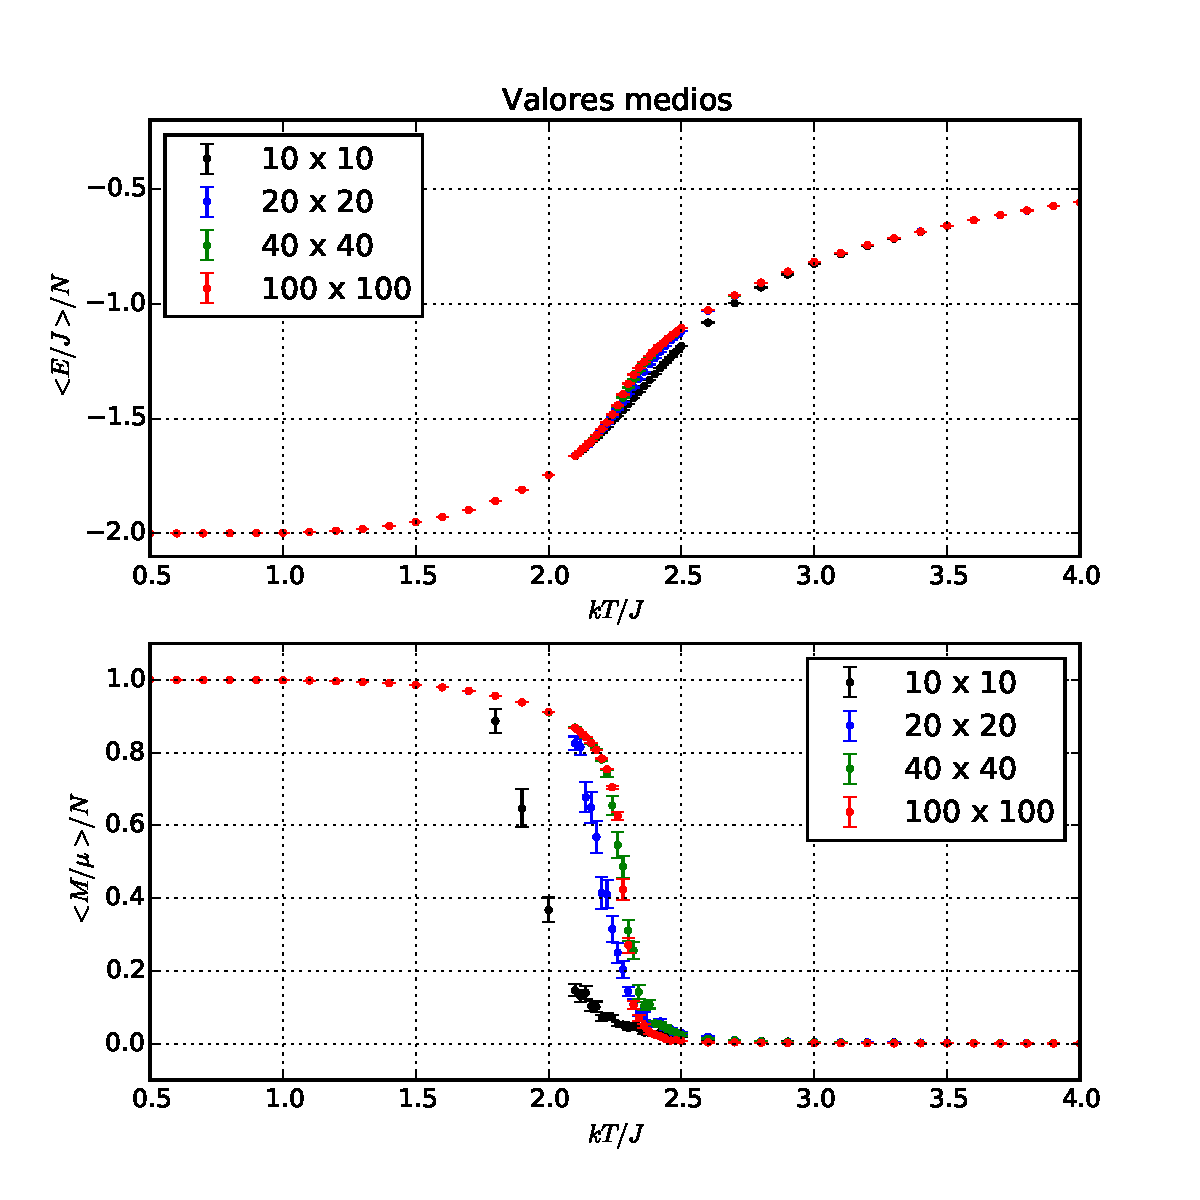
\includegraphics[scale=0.7]{tamano_val_medios.pdf} \\
      \caption{Energía y magnetización por spin para redes de spin de distinto 
      tamaños}\label{fig:tam_val_medios}
    \end{center}
\end{figure}

Como primera observación, se puede decir que los efectos de borde resultan 
irrelevantes fuera de la zone carcana a la temperatura crítica. Los valores de 
energía ni siqueira cambiand demasiado en dicha zona. En cambio, la 
magnetización presenta mayores variaciones para las distintas redes, 
principalmente en las redes de 10x10 y 20x20. Sin embargo, la diferencia se 
vuelve muy exigua al comparar las redes de 40x40 y 100x100 donde los efectos de 
borde no parece ser relevantes para la magnetización.

En la Figura \eqref{fig:tam_fluctuaciones} se muestran los resultados obtenidos 
del calor específico y suceptibilidad magnética para los cuatro tamaños 
simulados. Al igual con con $E$ y $M$, aquí los efectos de borde son más 
notorios cerca de la temperatura crítica.

La principal diferencia que se observa es que a medida que se aumenta el 
tamaño, el efecto de la divergencia en $T_c$ se hace más evidente. Las curvas 
son suaves para las redes de menor tamaño, mientras que se vuelven más 
puntiagudas para las redes de mayor tamaño. La diferencia entre las redes de 
40x40 y 100x100 se hacen notorias sólo muy cerca de la $T_c$ donde los valores 
de la última de ellas aumentan a más del doble.

\begin{figure}[H]
    \begin{center}
      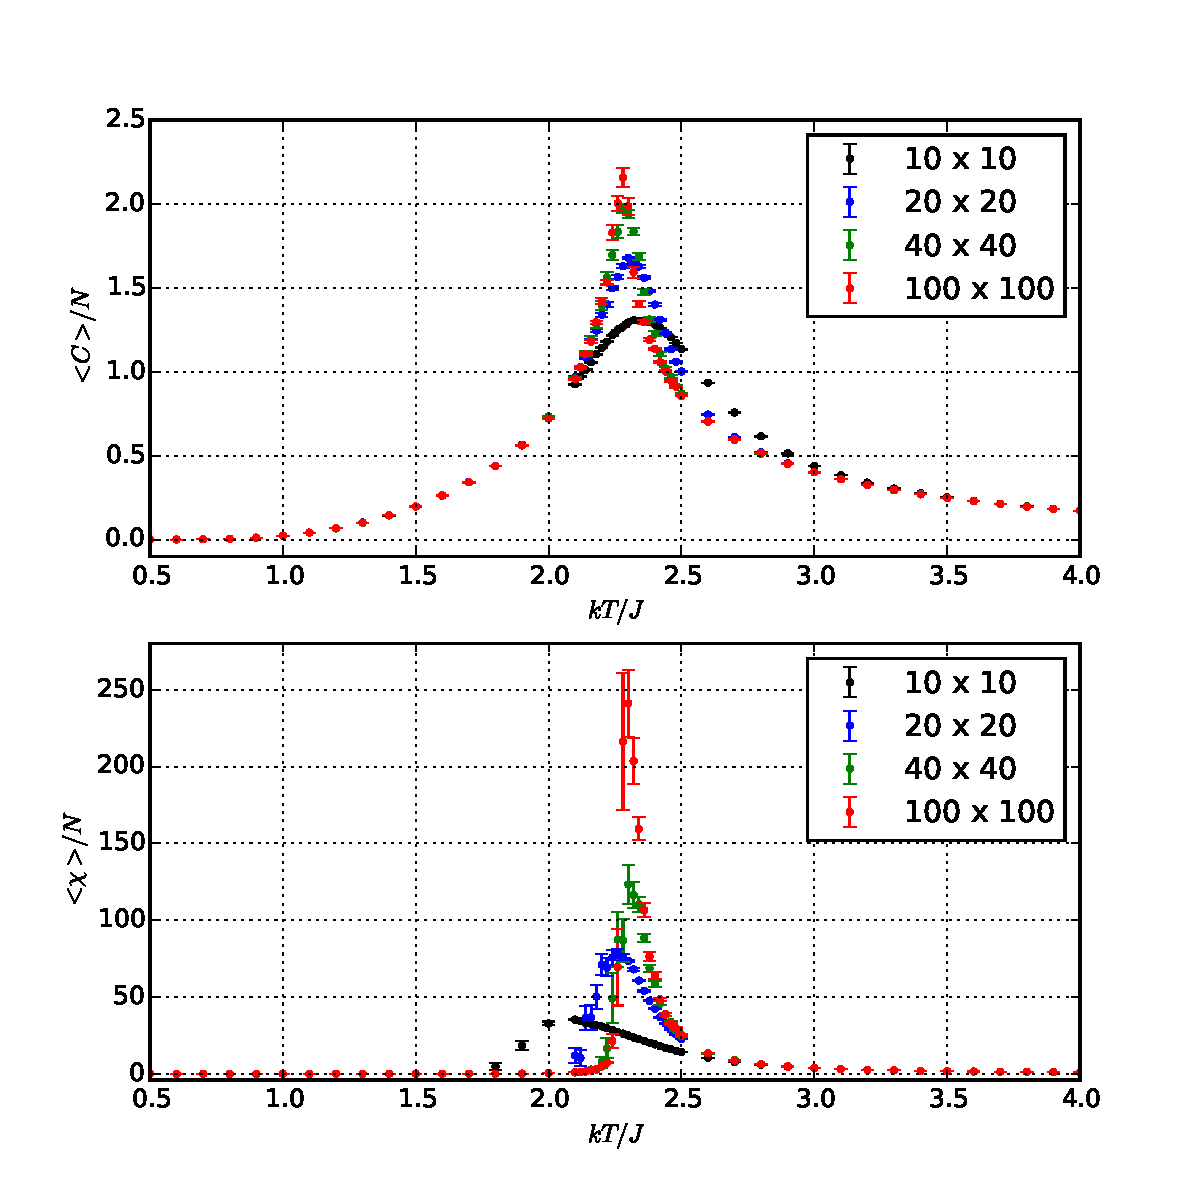
\includegraphics[scale=0.7]{tamano_fluctuaciones.pdf} \\
      \caption{Calor específico y suceptibilidad magnética por spin para redes 
      de spin 
      de distintos tamaños}\label{fig:tam_fluctuaciones}
    \end{center}
\end{figure}

%\begin{figure}[H]
%    \begin{center}
%      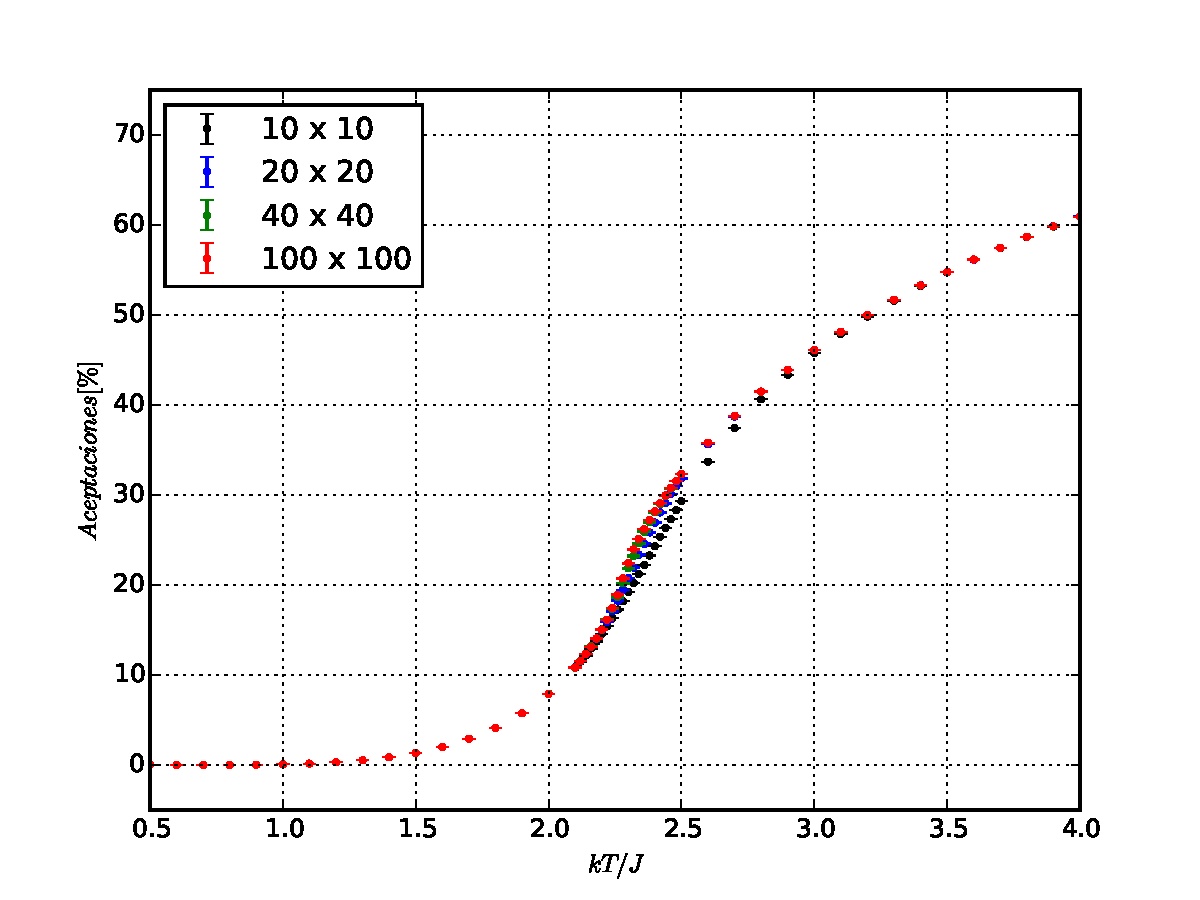
\includegraphics[scale=0.5]{tamano_aceptaciones.pdf} \\
%      \caption{Porcentaje de aceptaciones en el algoritmo de Metrópolis para 
%      redes de spin de distintos tamaños}\label{fig:tam_aceptaciones}
%    \end{center}
%\end{figure}

\subsection{Correlaciones temporales de la energía}

\begin{equation}\label{eq:corr_teo}
C_{EE}(\tau) = \frac{\langle \left[E(t+\tau)-\langle 
E\rangle\right]\left[E(t)-\langle E \rangle\right] \rangle
}{\langle E^2\rangle - \langle E \rangle ^2}
\end{equation}

El estimador utilizado para obtener la autocorrelación de la muestra discreta 
de datos fue:

\begin{equation}\label{eq:corr_est}
C_{EE}[k] = \frac{1}{\sigma^2(N_b-k)} \sum_{i=1}^{N_b - k}\left(E[i+k] - 
\langle E \rangle\right)\left(E[i]-\langle E\rangle\right)
\end{equation}

\noindent donde $N_b$ es la cantdiad de puntos presentes en el bloque de datos 
seleccionado. El valor informado consistió en dividir la historia temporal de 
$E[i]$ en $N_b$ bloques, calcular la auto-correlación con \eqref{eq:corr_est} 
en cada uno de ellos, y posteriormente calcular el promedio y desviación 
estandar:

\begin{subequations}
\begin{align}
\langle C_{EE}[k]\rangle &= \frac{1}{N_b} \sum_{b=1}^{N_b} C_{EE}[k]\\
\sigma(\langle C_{EE}[k]\rangle) &= \frac{\sigma(C_{EE}[k])}{\sqrt{N_b}}
\end{align}
\end{subequations}

Finalmente, asumiendo un modelo exponencial para la función de 
auto-correlación, se linealizaron los datos para realizar un ajuste y obtener 
el tiempo de correlación $\tau_c$ del sistema:

\begin{equation}
C_{EE}[k]=A e^{-t[k]/\tau_c} \qquad \Rightarrow \quad ln\left(C_{EE}[k]\right) 
= ln(A) - \frac{t[k]}{\tau_c}
\end{equation}

\subsection{Análisis de los resultados del cálculo de las correlaciones}

Aplicando la ecuación  \ref{eq:corr_est}  para el estimador de la 
autocorrelación de la muestra discreta
se calcularon autocorrelaciones a distintas temperaturas y con distintos 
tamaños 
de matriz de espines. Se agruparon los resultados de manera de mostrar en un 
mismo
tamaño de matriz, diferentes temperaturas y en iguales temperaturas distintos 
tamaños de matriz.

\subsubsection{Correlación en función de la temperatura}

En la figura \ref{fig:corre_20x20}, se pueden ver los resultados del cálculo
de correlaciones para  temperaturas $T =9.0 $, $T = 1.0 $, $T =0.8 $ y $T = 2.3 
$, en una matriz de tamaño 20x20.
En este caso con el descenso de la temperatura se observa un aumento del valor 
del parámetro
de correlación $\tau_{c}$.


\begin{figure}[h]
   \begin{center}
        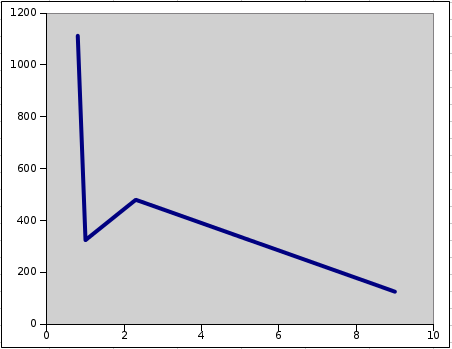
\includegraphics[scale=0.6]{corre_temperature.png} \\
        \caption{Parámetro de correlación  $\tau_{c}$ en función de la 
        temperatura $T$}\label{fig:corre_tempe}
    \end{center}
\end{figure}


\subsubsection{Correlación en función del tamaño del problema}
En las figuras \ref{fig:corre_tamano_t2} y \ref{fig:corre_tamano_t9}, se pueden 
ver los resultados del cálculo
de correlaciones para los tamaños de matriz 20x20 y 100x100 para valores de $T 
= 2.3$  y $T = 9.0$. 
En los dos casos se observa un aumento del parámetro de correlación con el 
aumento del 
tamaño de la matriz de spines.




\begin{figure}[H]
    \begin{center}
      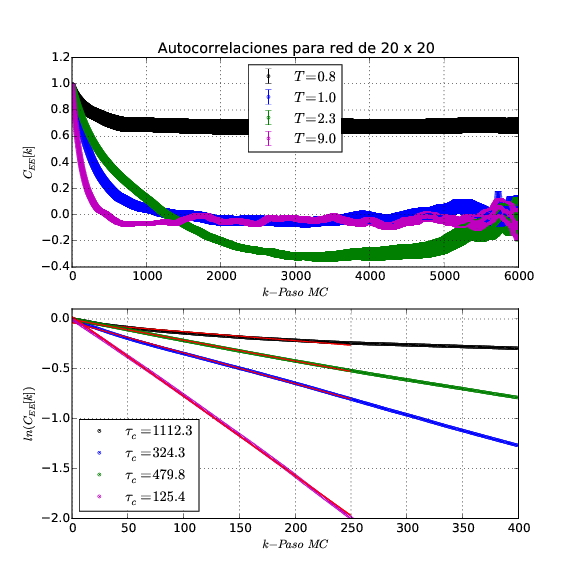
\includegraphics[scale=0.5]{corre_20x20.png} \\
      \caption{Funciones de auto-correlación temporales de la energía con su 
      banda de error para distintas temperaturas (arriba). Ajuste lineal en el 
      primer tramo de las funcione para obtener el tiempo de correlación 
      (abajo)}\label{fig:corre_20x20}
    \end{center}
\end{figure}

\begin{figure}[H]
\begin{center}
\hspace{-4em}
\begin{subfigure}{.49\textwidth}
    \begin{center}
      \includegraphics[scale=0.48]{{corre_tamano_t2.3}.png} \\
      \caption{$T=2.3$}\label{fig:corre_tamano_t2}
    \end{center}
\end{subfigure}
\begin{subfigure}{.49\textwidth}
    \begin{center}
      \includegraphics[scale=0.48]{{corre_tamano_t9.0}.png} \\
      \caption{$T=9.0$}\label{fig:corre_tamano_t9}
    \end{center}
\end{subfigure}
\caption{Funciones de autocorrelación temporal de la energía, con los valores 
del tiempo de correlación obtenidos. Se comparan distintos tamaños de redes a 
distintas temperaturas}
\end{center}
\end{figure}

%\begin{figure}[H]
%    \begin{center}
%      \includegraphics[scale=0.5]{{corre_tamano_t9.0}.png} \\
%      \caption{aaa}\label{fig:corre_tamano_t9}
%    \end{center}
%\end{figure}


%\inputencoding{utf8}
\section {Evoluci\'on de la matriz de estado de spines en funci\'on de la 
temperatura}


Al final de cada ciclo de c\'alculo, en cada una de las  temperaturas, se 
obtiene
la matriz de estado de los spines del sistema.

Un script en python recorre cada una de las carpetas, lee el archivo 
ultimo\_estado.txt,
que graba el programa ising, lo convierte a un array 2D de numpy, para luego 
con la 
librer\'ia matplotlib convertirlo a imagen y grabarlo en disco. 
Luego de grabado en disco con el programa ffmpeg, se obtiene un video que 
muestra
la secuencia de la evoluci\'on del sistema desde temperaturas altas a bajas.



Las figuras \ref{fig:Talta}, \ref{fig:Tmedia},  \ref{fig:Tbaja},  
%\ref{fig:frame2.0},  \ref{fig:frame1.3},  \ref{fig:frame0.5}, 
muestran algunas im\'agenes de esa secuencia correspondientes a  estados
del sistema a temperaturas altas, medias y bajas respectivamente, 
T: 5.0, 3.8, 2.3, 2.0, 1.3 y 0.5.

Al disminuir la temperatura se observa la tendencia a que un valor de spin
tenga m\'as presencia sobre la matriz que el otro. En temperaturas bajas el
spin que mostraba tendencia mayoritaria a temperaturas m\'as altas, termina
siendo el único spin presente en la matriz.




\begin{figure}[H]
	\centering
\begin{subfigure}{.49\textwidth}
	\centering
      \includegraphics[scale=0.3]{{frame5.0}.pdf} \\
      \caption{Temperatura 5.0}\label{fig:frame5.0}
\end{subfigure}
\begin{subfigure}{.49\textwidth}
	\centering
      \includegraphics[scale=0.3]{{frame3.8}.pdf} \\
      \caption{Temperatura 3.8}\label{fig:frame3.8}
\end{subfigure}
      \caption{Temperaturas altas}\label{fig:Talta}
\end{figure}

\begin{figure}[H]
	\centering
\begin{subfigure}{.49\textwidth}
	\centering
      \includegraphics[scale=0.3]{{frame2.3}.pdf} \\
      \caption{Temperatura 2.3}\label{fig:frame2.3}
\end{subfigure}
\begin{subfigure}{.49\textwidth}
	\centering
      \includegraphics[scale=0.3]{{frame2.0}.pdf} \\
      \caption{Temperatura 2.0}\label{fig:frame2.0}
\end{subfigure}

\caption{Temperaturas medias}\label{fig:Tmedia}
\end{figure}

\begin{figure}[H]
	\centering
\begin{subfigure}{.49\textwidth}
	\centering
      \includegraphics[scale=0.3]{{frame1.3}.pdf} \\
      \caption{Temperatura 1.3}\label{fig:frame1.3}
\end{subfigure}
\begin{subfigure}{.49\textwidth}
	\centering
      \includegraphics[scale=0.3]{{frame0.5}.pdf} \\
      \caption{Temperatura 0.5}\label{fig:frame0.5}
\end{subfigure}

\caption{Temperaturas bajas}\label{fig:Tbaja}
\end{figure}


\section{Conclusiones}

Se simuló el modelo de Ising en 2D utilizando el algoritmo de Metrópolis. Se 
escribieron los programas en lenguaje Fortran para el cálculo principal y se 
utilizó Python para manejar la ejecución y procesamiento de los datos. Con los 
scripts de python fue posible ejecutar barridos de temperatura tanto en forma 
serial como paralelizada.

De las simulaciones realizadas se obtuvieron las variables físicas más 
relevantes del sistema en función de la temperatura. Se analizó el efecto de 
borde analizando distintos tamaños de la red de spines. Se comprobó que para 
las magnitudes estudiadas, no existía mucha diferencia entre las redes de 40x40 
y 100x100. Se analizaron también los tiempos de correlación existentes en la 
simulación para distintas temperaturas y distintos tamaños de las redes.


\begin{thebibliography}{9}

\bibitem{chand1987}
  David Chandler,
  Introduction to modern statistical mechanics,
  Oxford University Press, Massachusetts,
  Vol. 1,
  1987.

\end{thebibliography}
\end{document}
